\documentclass{article}
\author{Pranav Chandra \\ 2023AAPS0013P}
\title{Communication Systems Lab 1}

%Packages
\usepackage{listings}
\usepackage{graphicx}
\usepackage{subcaption}
\usepackage{listings}
\usepackage{xcolor}

\definecolor{codegreen}{rgb}{0,0.6,0}
\definecolor{codegray}{rgb}{0.5,0.5,0.5}
\definecolor{codepurple}{rgb}{0.58,0,0.82}
\definecolor{backcolour}{rgb}{0.95,0.95,0.92}

\lstdefinestyle{mystyle}{
    backgroundcolor=\color{backcolour},   
    commentstyle=\color{codegreen},
    keywordstyle=\color{magenta},
    numberstyle=\tiny\color{codegray},
    stringstyle=\color{codepurple},
    basicstyle=\ttfamily\footnotesize,
    breakatwhitespace=false,         
    breaklines=true,                 
    captionpos=b,                    
    keepspaces=true,                 
    numbers=left,                    
    numbersep=5pt,                  
    showspaces=false,                
    showstringspaces=false,
    showtabs=false,                  
    tabsize=2
}

\lstset{style=mystyle}

\begin{document}
	\maketitle
	\section{Question 1}
	\textbf{Question: } Generate a rectangular waveform using the fourier series expansion of a rectangular wave at $f_0 = 50 Hz$.
	\begin{equation}
		m(t) = \frac{4}{\pi} \sum_{n - 1, 3, 5...}^{N} \frac{1}{n} \sin(2\pi n f_0 t) 
	\end{equation}
	Plot the time domain $m(t)$ and frequency domain $|M(f)|$ for different $N$.
	
	\textbf{Answer:}
	This is a relatively simple problem. It was sovled in MATLAB. Sampling frequency was set to 2$\times$ the maximum frequency $N\times f_0$. 
	After running the code, figures \ref{fig:time domain image} and \ref{fig:freq domain image} were generated for the time domain and frequency domain signals.

	The code for this question can be found in Appendix \ref{app:question 1 code}.
	\begin{figure}
		\centering
		\begin{subfigure}[b]{0.45\textwidth}
			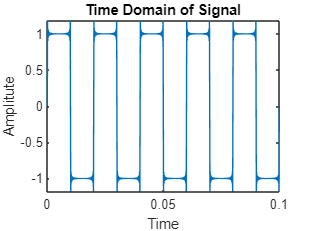
\includegraphics[width=\textwidth]{l1_q1_media/figure_0.png}
			\caption{Time Domain Image, $N = 100$}
			\label{fig:time domain image}
		\end{subfigure}
		\begin{subfigure}[b]{0.45\textwidth}
			\centering
			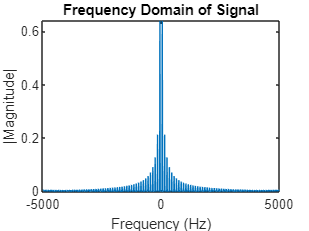
\includegraphics[width=\textwidth]{l1_q1_media/figure_1.png}
			\caption{Frequency Domain Graph}
			\label{fig:freq domain image}
		\end{subfigure}
		\caption{Graphs From Question 1}
	\end{figure}

	\newpage

	\section{Question 2}
	\textbf{Question: } Generate a periodic rectangular pulse of period 20ms using the built-in square function and plot its waveform in the time domain and frequency spectrum using fft. Then, pass the rectangular pulse through a low-pass filter with impulse response 2Bsinc(2Bt) and observe the output in the frequency domain for different values of B. Use the convolution operation.


	This is another line that I'm going to type here.

	
	\textbf{Answer: }
	Using the square function, Figures \ref{fig:time original sq wave} and \ref{fig:freq original sq wave} were generated for the time domain and frequency domain representations. 

	The code for this question can be found in Appendix \ref{app:question 2 code}.
	\begin{figure}[h!]
		\centering
		\begin{subfigure}[b]{0.45\textwidth}
			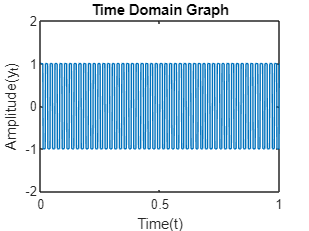
\includegraphics[width=\textwidth]{l1_q1_media/figure_2.png}
			\caption{MATLAB Gen. Square Wave}
			\label{fig:time original sq wave}
		\end{subfigure}
		\hspace{2pt}
		\begin{subfigure}[b]{0.45\textwidth}
			\centering
			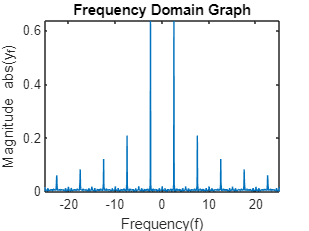
\includegraphics[width=\textwidth]{l1_q1_media/figure_3.png}
			\caption{Frequency Domain Representation}
			\label{fig:freq original sq wave}
		\end{subfigure}
		\caption{Graphs of the Square Wave}
	\end{figure}

	After this, a function \texttt{y\_convd} was created along with the variable $B$. Various values of $B$ were iterated upon and the filter was used on the original square wave using the \texttt{conv(a, b, 'same')} operation. Figure \ref{fig:conv sq wave} shows the effect of the convolution. Different values of $B$ and ranges of $t$ showed slightly different effects, but all of them contained the same structure.
	\begin{figure}[h!]
		\centering
		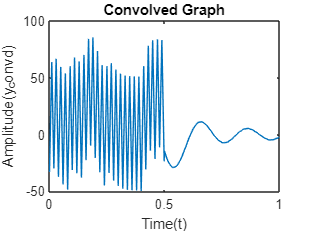
\includegraphics[width=0.45\linewidth]{l1_q1_media/figure_4.png}
		\caption{Convolved Function}
		\label{fig:conv sq wave}
	\end{figure}

	This concludes the first lab. Further labs will likely be done in Python as opposed to MATLAB.

	\appendix

	\section{Question 1 Code}
	\label{app:question 1 code}
	\begin{lstlisting}[language=Octave]
N = 100;
f = 50;
fs = 2*f*N;
dt = 1/(fs);
t = 0:dt:0.1;
m_t = zeros(size(t));

for n = 1:2:N
    m_t = m_t + (1/n)*(sin(2*pi*n*f*t));
end

m_t = (4/pi).*m_t;

m_f = fftshift(fft(m_t));
m_f = m_f/norm(m_f);
f_range = linspace(-fs/2, fs/2, length(m_f));

figure();
plot(t, m_t);
xlabel("Time");
ylabel("Amplitute")
title("Time Domain of Signal")

figure();
plot(f_range, abs(m_f));
xlabel("Frequency (Hz)");
ylabel("|Magnitude|");
title("Frequency Domain of Signal");
	\end{lstlisting}

	\newpage

	\section{Question 2 Code}
	\label{app:question 2 code}
	\begin{lstlisting}[language=Octave]
%Defining Variables
fs = 20*(1/20e-3);
t = 0:1/fs:1;
B = 5;
f = 1/20e-3;

%Calculating Square Wave
y_t = square(2*pi*f*t);

%Calculating FFT of Wave
y_f = fftshift(fft(y_t));
y_f = y_f / norm(y_f)
N = length(y_t);
f_rng = linspace(-f/2, f/2, N);

%Creating a convolved signal of y and the signal mentioned in the qn
conv_func = 2*B*sinc(2*B*t);
y_convd = conv(y_t, conv_func, 'same');

%Plotting the various waves
figure();
plot(t,y_t);
xlabel("Time(t)");
ylabel("Amplitude(y_t)");
ylim([-2 2])
title("Time Domain Graph");

figure();
plot(f_rng, abs(y_f));
xlabel("Frequency(f)");
ylabel("Magnitude abs(y_f)");
title("Frequency Domain Graph");

%Plotting the convolved signal
figure();
plot(t, y_convd);
xlabel("Time(t)");
ylabel("Amplitude(y_convd)");
title("Convolved Graph");
	\end{lstlisting}
	
\end{document}
